\chapter{稳定磁场}
\section{作业习题}
\subsection*{一、填空题}
\begin{enumerate}
    \item 如图~\ref{fig:65},一个带电$Q$的粒子($Q>0$),以速度$V$向右运动,求距粒子$r$处产生的磁感应强度为$B=\nl$,方向为\nl.
    \begin{figure}[H]
        \centering
        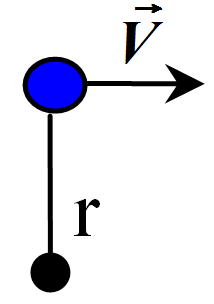
\includegraphics[width=0.25\textwidth]{fig65}
        \caption{如图所示}\label{fig:65}
    \end{figure}
    \item 一个无限长的圆形螺线管,单位长度匝数为$n$,通有电流强度$I$,则在螺线管内部的磁感应强度大小$B=\nl$.
    \item 如图~\ref{fig:66},一平面线圈由半径为~$R$~的1/4圆弧和相互垂直的二直线组成,通以电流$I$,把它放在磁感强度为~$B$~的均匀磁场中,则线圈磁矩大小$p_m=\nl$.
    \begin{figure}[H]
        \centering
        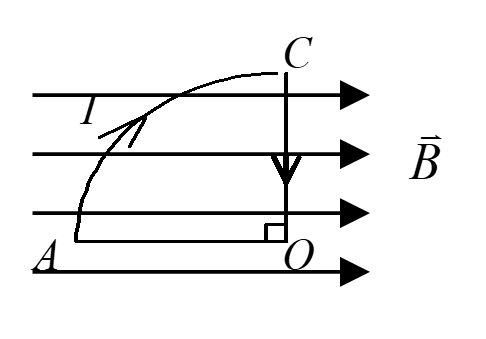
\includegraphics[width=0.25\textwidth]{fig66}
        \caption{如图所示}\label{fig:66}
    \end{figure}
    \item 如图~\ref{fig:67}, 真空中环绕两根通有电流为$I$的导线的两种环路,则对环路$L_1$有$\oint_{l1}\vec{B}\cdot \mathrm{d}\vec{l}=\nl$,对环路$L_2$有$\oint_{l2}\vec{B}\cdot \mathrm{d}\vec{l}=\nl$.
    \begin{figure}[H]
        \centering
        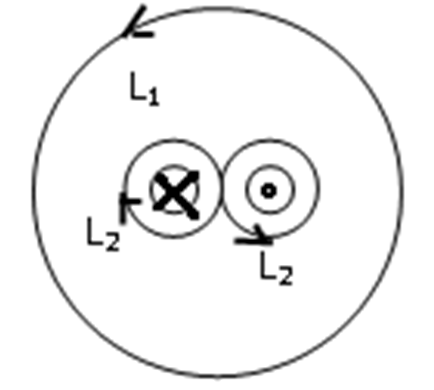
\includegraphics[width=0.25\textwidth]{fig67}
        \caption{如图所示}\label{fig:67}
    \end{figure}
    \item 在安培环路定理$\oint_{l} \vec{B}\cdot \mathrm{d}\vec{l}$中, $\sum \mathbf{I_i}$是指\nl;$\vec{B}$~是指\nl;它是由\nl 决定的.
    \item 一半径为$a$的无限长直载流导线,沿轴向均匀地流有电流$I$,若作一个半径为$R=5a$,高为$L$的柱形曲面,已知柱形曲面的轴与载流导线的轴平行且相距$3a$,如图~\ref{fig:68},则$B$在圆柱侧面$S$上的积分~$\int_S \vec{B}\cdot \mathrm{d} \vec{S}$.
    \begin{figure}[H]
        \centering
        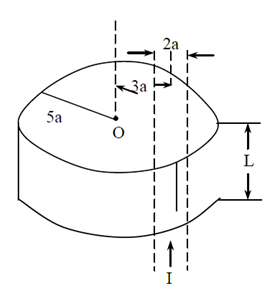
\includegraphics[width=0.25\textwidth]{fig68}
        \caption{如图所示}\label{fig:68}
    \end{figure}
    \item 通有电流$I$ 的长直导线在一平面内被弯成如图~\ref{fig:69}~形状($R$为已知),放于垂直进入纸面的均匀磁场$\vec{B}$中,则整个导线所受的安培力大小$F=\nl$.
     \begin{figure}[H]
        \centering
        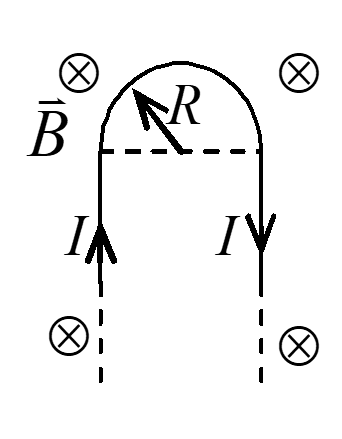
\includegraphics[width=0.25\textwidth]{fig69}
        \caption{如图所示}\label{fig:69}
    \end{figure} 
    \item 如图所示~\ref{fig:70},平行放置在同一平面内的三条载流长直导线,电流依次是$I$,$I$,$2I$要使导线$AB$所受的安培力等于零,则
    $x=\nl$.
    \begin{figure}[H]
        \centering
        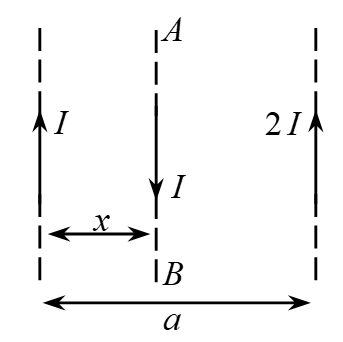
\includegraphics[width=0.25\textwidth]{fig70}
        \caption{如图所示}\label{fig:70}
    \end{figure}
\end{enumerate}
\subsection*{二、选择题}
\begin{enumerate}
    \item 长直导线通有电流$I$,将其弯成如图所示\ref{fig:71}形状,则$O$点处的磁感应强度大小为~\spaces
    \twoch{$\frac{\mu_0I}{2\pi R}+\frac{\mu_0 I}{4R}$}{$\frac{\mu_0 I}{4\pi R}+\frac{\mu_0 I}{8R}$}{$\frac{\mu_0 I}{2\pi R}+\frac{\mu_0 I}{8 R}$}{$\frac{\mu_0 I}{4\pi R}+\frac{\mu_0 I}{4 R}$}
    \insertfig{0.25}{fig71}{fig:71}
    \item 一根载有电流$I$的无限长直导线,在$A$处弯成半径为$R$的圆形,由于导线外有绝缘层,在$A$处两导线并不短路,则在圆心处磁感应强度$\vec{B}$的大小为~\spaces
    \twoch{$I(\mu_0 +1 )/(2\pi R)$}{$\mu_0 \pi I / (2\pi R)$}{$\mu I (1+\pi R)$}{$\mu_0 I (1+\pi)/(4\pi R)$}

    \item 四条相互平行的载流长直导线电流强度均为$I$,方向如图\ref{fig:73}。设正方形的边长为$2a$,则正方形中心的磁感应强度为~\spaces
    \fourch{$\frac{2\mu_0}{\pi a}I$}{$\frac{2\mu_0}{\sqrt{2}\pi a}I$}{$\frac{\mu_0}{\pi a}I$}{$0$}
    \insertfig{0.25}{fig72}{fig:72}
    \item 如图\ref{fig:73}, 在磁感强度为$\vec{B}$的均匀磁场中作一半径为$r$的半球面$S$,$S$边线所在平面的法线方向单位矢量$\vec{n}$与$\vec{B}$的夹角为$\alpha$,则通过半球面$S$的磁通量(取弯面向外为正)为~\spaces
    \fourch{$\pi r^2 B$}{$2\pi r^2 B$}{$-\pi r^2 B \mathrm{sin} \alpha$}{$-\pi r^2 B\mathrm{cos}\alpha$}
    \insertfig{0.25}{fig73}{fig:73}
    \item 如图\ref{fig:74},两根直导线~$ab$~和~$cd$~沿半径方向被接到一个截面处处相等的铁环上,稳恒电流$I$从$a$端流入而从$d$端流出,则磁感强度$\vec{B}$沿图中包围铁环截面的闭合路径$L$的积分$\oint_L \vec{B}\cdot \dd \vec{l}$等于~\spaces
    \fourch{$\mu_0I$}{$-\mu_0 I/3$}{$2\mu_0I/3$}{$-2\mu_0 I/3$}
    \insertfig{0.25}{fig74}{fig:74}
    \item 如图所示\ref{fig:75},流出纸面的电流为$2I$,流进纸面的电流为$I$,则下述式中哪一个是正确的是~\spaces
    \twoch{$\oint_{L1}\vec{B}\cdot \dd \vec{l}=2\mu_0 I$}{$\oint_{L2}\vec{B}\cdot \dd \vec{l}=\mu_0 I$}{$\oint_{L3}\vec{B}\cdot \dd \vec{l}=-\mu_0 I$}{$\oint_{L4}\vec{B}\cdot \dd \vec{l}=-\mu_0 I$}
    \insertfig{0.25}{fig75}{fig:75}
    \item 如图~\ref{fig:76}~六根互相绝缘导线,通以电流强度均为$I$,区域$I$、$II$、$III$、$IV$均为正方形,那么指向纸内的磁通量最大的区域是~\spaces
    \fourch{$I$区域}{$II$区域}{$III$区域}{$IV$区域}
    \insertfig{0.25}{fig76}{fig:76}
    \item 无限长直导线通有电流$I$,右侧有两个相连的矩形回路,分别是$S_1$和$S_2$,则通过两个矩形回路$S_1$、$S_2$的磁通量之比为~\spaces
    \fourch{1:2}{1:1}{1:4}{2:1}
    \insertfig{0.25}{fig77}{fig:77}
\end{enumerate}
\subsection*{三、计算题}
\begin{enumerate}
    \item 载有电流为$I$的无限长导线,弯成如图~\ref{fig:78}~形状,其中一段是半径为$a$的半圆,求圆心处的磁感应强度$\vec{B}$的大小.
    \insertfig{0.25}{fig78}{fig:78}
    \item 如图~\ref{fig:79}~半径为$R$的带电圆盘,电荷面密度为$\sigma$,圆盘以角速度$\omega$绕过盘心并垂直盘面的轴旋转,求中心$O$处的磁感应强度$\vec{B}$。
    \insertfig{0.25}{fig79}{fig:79}
    \item 如图~\ref{fig:80}一半径为$R$的无限长圆柱形导体,现有电流$I$均匀地流过导体横截面,且电流方向与导体轴线平行,求空间的磁场分布。
    \insertfig{0.25}{fig80}{fig:80}
    \item 如图~\ref{fig:81}~在载流为$I_1$的长直导线旁,共面放置一载流为$I_2$的等腰直角三角形线圈$abc$,腰长$ab=ac=L$,边长$ab$平行于长直导线,相距$L$,求线圈各边受的磁力$F$.
    \insertfig{0.25}{fig81}{fig:81}
    \item 如图~\ref{fig:82}无限长直导线和半径为$R$的圆形线圈,彼此绝缘,共面放置,且圆线圈直径和直导线重合,直导线与圆线圈分别通以电流$I_1$和$I_2$,求
    \begin{enumerate}[label=(\arabic*)]
        \item 长直导线对半圆弧$abc$所作用的磁力;
        \item 整个圆形线圈所受的磁力.
    \end{enumerate}
    \insertfig{0.25}{fig82}{fig:82}
\end{enumerate}